% This must be in the first 5 lines to tell arXiv to use pdfLaTeX, which is strongly recommended.
\pdfoutput=1
% In particular, the hyperref package requires pdfLaTeX in order to break URLs across lines.

\documentclass[11pt]{article}

% Remove the "review" option to generate the final version.
\usepackage{acl}

% Standard package includes
\usepackage{times}
\usepackage{latexsym}

% For proper rendering and hyphenation of words containing Latin characters (including in bib files)
\usepackage[T1]{fontenc}
% For Vietnamese characters
% \usepackage[T5]{fontenc}
% See https://www.latex-project.org/help/documentation/encguide.pdf for other character sets

% This assumes your files are encoded as UTF8
\usepackage[utf8]{inputenc}

% This is not strictly necessary, and may be commented out,
% but it will improve the layout of the manuscript,
% and will typically save some space.
\usepackage{microtype}

% Nicer enumerations:
\usepackage{enumitem}
% lets us use footnotes in tables
\usepackage{tablefootnote}

% provides the \ex command to make linguistics-style numbered examples
\usepackage{gb4e}
% recommended by https://tex.stackexchange.com/questions/325621/gb4e-package-causing-capacity-errors
\noautomath

% much prettier tables:
\usepackage{booktabs}
\usepackage[singlelinecheck=false]{caption} 

\usepackage{caption}
\usepackage{graphicx, subfig}
\usepackage{multirow}
\newcommand{\hey}[1]{\textcolor{blue}{\textbf{#1}}}


\title{Probing for Understanding of English Verb Classes and Alternations in Large Language Models}

% Author information can be set in various styles:
% For several authors from the same institution:
% \author{Author 1 \and ... \and Author n \\
%         Address line \\ ... \\ Address line}
% if the names do not fit well on one line use
%         Author 1 \\ {\bf Author 2} \\ ... \\ {\bf Author n} \\
% For authors from different institutions:
% \author{Author 1 \\ Address line \\  ... \\ Address line
%         \And  ... \And
%         Author n \\ Address line \\ ... \\ Address line}
% To start a seperate ``row'' of authors use \AND, as in
% \author{Author 1 \\ Address line \\  ... \\ Address line
%         \AND
%         Author 2 \\ Address line \\ ... \\ Address line \And
%         Author 3 \\ Address line \\ ... \\ Address line}

\author{James V.~Bruno, Jiayu Han, David K.~Yi, Peter Zukerman \thanks{ The authors' names appear in alphabetical order.}\\
The University of Washington\\
  \texttt{\{jbruno, jyhan126, davidyi6, pzuk\}@uw.edu}}

\begin{document}
\maketitle
\begin{abstract}
Abstract goes here, man.
\end{abstract}

\section{Introduction}
We investigate the extent to which alternation class membership is represented in the word and sentence embeddings produced by BERT \citep{bertpaper}.  As first comprehensively cataloged by \citet{levin1993}, verbs pattern together into classes according to the syntactic alternations in which they can and cannot participate.  For example, (\ref{ex:good-caus-inch}) illustrates the \emph{causative-inchoative} alternation.  \emph{Break} can be a transitive verb in which the subject of the sentence is the agent and the direct object is the theme, as in example (1a).  It can also alternate with the form in (1b), in which the subject of the sentence is the theme and the agent is unexpressed. % TODO: figure out how to make those references work properly.
However, (\ref{ex:bad-caus-inch}) demonstrates that \emph{cut} cannot participate in the same alternation, despite its semantic similarity.

\begin{exe}
    \ex
        \label{ex:good-caus-inch}
        \begin{xlist}
            \ex[] {Janet broke the cup.}
            \ex[] {The cup broke.}
        \end{xlist}

    \ex
        \label{ex:bad-caus-inch}
        \begin{xlist}
            \ex[]{Margaret cut the bread.}
            \ex[*]{The bread cut.}
        \end{xlist}
\end{exe}

(\ref{ex:good-spray-load}) demonstrates an alternation of a different class -- namely, the \emph{spray-load} class, in which the theme and locative arguments can be syntactically realized as either direct objects or objects of the preposition.  \emph{Spray} can participate in the alternation, but as shown in (\ref{ex:bad-spray-load}), \emph{pour} cannot.

\begin{exe}
    \ex 
        \label{ex:good-spray-load}
        \begin{xlist}
            \ex[] {Jack sprayed paint on the wall.}
            \ex[] {Jack sprayed the wall with paint.}
        \end{xlist}

    \ex 
        \label{ex:bad-spray-load}
        \begin{xlist}
            \ex[] {Tamara poured water into the bowl.}
            \ex[*] {Tamara poured the bowl with water.}
        \end{xlist}
\end{exe}

The alternations in which a verb may participate is taken to be a lexical property of the verb \citep[e.g.][]{pinker1989,levin1993,levin1995unaccusativity,shafer2009causative}.  Moreover, the alternations should be observable in large corpora of texts, and are therefore available as training data during the Masked-Language-Modeling task used to train neural language models such as BERT.  Negative examples such as (2b) and (4b) should be virtually absent from the training data.  This leads us to hypothesize that BERT representations may encode whether particular verbs are allowed to participate in syntactic alternations of various classes.  Our research questions are as follows:

\begin{enumerate}
    \item Do BERT's token-level representations encode information about which syntactic frames an individual verb can participate in?
    \item At the sentence level, do BERT's layers represent the frame and alternation properties of their main verb?
    
\end{enumerate}

\hey{We'll have to modify the below once it's clear how we're presenting the control task work and data generation.}
After a brief review of related literature in Section~\ref{sec:litreview}, we present our datasets in Section~\ref{sec:data}.  We then present \hey{how many} experiments to answer our research questions in Sections~\ref{sec:experiment1}~and~\ref{sec:experiment2}.  Each of these sections have independent Method and Results sections.  Finally, we offer a discussion in Section~\ref{sec:discussion} and overall conclusions in Section~\ref{sec:conclusion}.

\section{Related work}
\label{sec:litreview}
\hey{David, this is just a copy-and-paste from the proposal. -JB}
Our work follows \citet{kann-etal-2019-verb}, who attempt to predict verb-classes on the basis of GloVe embeddings \citep{glove} and embeddings derived from the 100M-token British National Corpus with the intentionally simple single-directional LSTM of \citealt{warstadt2019neural}.  They also attempt to use the same LSTM to predict sentence grammaticality.  Because their primary research focus has to do with how neural language models can inform learnability (in the sense of human language acquisition), they use language models derived from ``an amount of data similar to what humans are exposed to during language acquisition'' and intentionally avoid models trained on ``several orders of magnitude more data than humans see in a lifetime'' (p. 291).  They also use a multi-layer perceptron with a hidden layer to predict alternation classes.  

As described in Section \ref{sec:experiment1}, we depart from \citealt{kann-etal-2019-verb} and build on it by examining the embedding representations of BERT which are derived from a training corpus of $3.3$ billion words. We then use a simple linear diagnostic classifier to probe the representations, as our research questions focuses on the BERT embeddings themselves.

Finally, we note that \citet{kann-etal-2019-verb} achieved only modest performance in raw prediction accuracy, and only for a limited number of verb classes.  While this was a valuable result for their research goals, our hypothesis is that we may achieve higher prediction accuracy due to BERT's more complex architecture and the larger size of its training data.

To our knowledge, attempting to predict a variety of verb classes along the lines of \citealt{levin1993} from BERT representations is novel.  Apart from \citealt{kann-etal-2019-verb}, the closest related work is \citealt{causativity-neurons}, which uses diagnostic classifiers to probe representations of causativity, and \citealt{thrush2020investigating}, which examines BERT's few-shot learning capabilities in an alternation-class prediction task in which the verbs are nonce words.


\section{Data}
\label{sec:data}
\hey{Just flagging this section for Peter.  Not sure if data generation should go here or someplace else.}
We use three datasets. First, we take advantage of the two datasets of \citet{kann-etal-2019-verb}.  One is the \textbf{L}exic\textbf{a}l \textbf{V}erb-frame \textbf{A}lternations dataset (LaVA), which is based on \citet{levin1993}.  It contains a mapping of $516$ verbs to $5$ alternation classes, which are further subdivided based on specific properties of each alternation.  The broad categories of the alternation classes are: \emph{Spray-Load}, \emph{Causative-Inchoative}, \emph{Dative}, \emph{There-insertion}, and \emph{Understood-object}.  The other dataset is the \textbf{F}rames and \textbf{A}lternations of \textbf{V}erbs \textbf{A}cceptability (FAVA) dataset, a corpus of $9,413$ semi-automatically generated sentences formed from the verbs in LaVa, along with human grammaticality judgments. Furthermore, we provide an extended dataset based on FAVA, FAVA-ex, which widens the scope of verbs and uses 1591 verbs from the 5 broad alternation categories in \citet{levin1993}. The corpus consists of $2982$ semi-automatically generated sentences along with human grammaticality judgments. 

\section{Experiment 1: Word-embeddings}
\label{sec:experiment1}

\subsection{Method}
In order to answer the first question, \textit{Do BERT's token-level representations encode information about which syntactic frames an individual verb can participate in?}, we build one diagnostic classifier for each syntactic frame.  For example, to probe the \textit{spray-load} alternation, we build two classifiers: one that predicts whether a verb can participate in the  frame exemplified by \textit{spray paint on the wall}, that is, the \textit{locative} frame; and one that predicts whether a verb can participate in the frame exemplified by \textit{spray the wall with paint}, that is, the \textit{preposition} frame.  

Futhermore, we build distinct classifiers for each layer of BERT using \texttt{bert-base-uncased} as implemented in the \texttt{HuggingFace} python package \citep{huggingface}.  For the word-embedding layer (hereafter the \textit{static} embeddings), the input to the classifiers is average of the embeddings from the word pieces from the bottom layer.  The embeddings are from each of the $516$ verbs in the FAVA dataset.  For layers 1--12 (hereafter the \textit{contextual} embeddings), the input to the classifiers is formed from the the $6,137$ grammatical sentences from the LaVA dataset.  For each verb frame, we input the corresponding grammatical sentences to BERT and, for each hidden layer, we take the average embedding for the token representation across all grammatical sentences.

The diagnostic classifier is a Logistic Regression classifier as implemented in \texttt{scikit-learn} \citep{sklearn}.  As our interest is in probing the extent to which alternation class membership is represented in the embeddings and we are not concerned with over-fitting, we do not apply an L2-penalty. Following \citet{kann-etal-2019-verb}, we use stratified 4-fold cross-validation due to the limited size of the dataset, and we calculate evaluation metrics on the combined predictions from the 4 models.

Also following \citet{kann-etal-2019-verb}, we report Matthews Correlation Co-efficient (MCC) \citep{mcc} in addition to accuracy.  MCC is better suited to data such as ours, in which there is an extreme majority class bias.


\subsection{Results}

\subsubsection{Static Word Embeddings}
\begin{table*}[!h]
\begin{tabular}{lrrrrr}
\toprule
{} & \multicolumn{3}{c}{MCC} & \multicolumn{2}{c}{Accuracy} \\ \cmidrule(r){2-4} \cmidrule(r){5-6}
{} &   \multicolumn{1}{c}{Reference} &  \multicolumn{1}{c}{BERT} & \multicolumn{1}{c}{$\Delta$} & 
 \multicolumn{1}{c}{Model} &   \multicolumn{1}{c}{Baseline}  \\
\midrule
\textsc{Causative-Inchoative} & & & & & \\
\hspace{1em} Inchoative   &    0.555 & 0.741 &      0.186 &     0.885 &  0.664 \\
\hspace{1em} Causative    &    0.000 & 0.000 &      0.000 &     1.000 &  1.000 \\
\textsc{Dative}&          &           &            &           &        \\
\hspace{1em} Preposition       &    0.320 & 0.701 &      0.381 &     0.925 &  0.853 \\
\hspace{1em} Double-Object     &    0.482 & 0.614 &      0.132 &     0.913 &  0.857 \\
\textsc{Spray-Load}&         &       &            &           &        \\
\hspace{1em} With              &    0.645 & 0.633 &     -0.012 &     0.848 &  0.706 \\
\hspace{1em} Locative          &    0.253 & 0.525 &      0.272 &     0.834 &  0.749 \\
\textsc{There\textsuperscript{*}}&         &       &            &           &        \\
\hspace{1em} No-There          &    0.000 & 0.000 &      0.000 &     1.000 &  1.000 \\
\hspace{1em} There             &    0.459 & 0.593 &      0.134 &     0.876 &  0.793 \\
\textsc{Understood Object }&         &       &            &           &        \\
\hspace{1em} Refl\textsuperscript{$\dagger$}    &    0.000 & 0.466 &      0.466 &     0.867 &  0.833 \\
\hspace{1em} Non-Refl        &    0.219 & 0.563 &      0.344 &     0.984 &  0.979 \\
\bottomrule
\end{tabular}
\caption{Results from Word-Level experiments with static embeddings. Reference MCC is from  \protect\citet{kann-etal-2019-verb}'s CoLA experiment.  Baseline refers to a Majority Baseline.  \textsuperscript{*}We strongly believe that \protect\citeauthor{kann-etal-2019-verb}}reversed the labels for \textit{There}, and we report what we believe to be correct. \textsuperscript{$\dagger$}There appears to be a small discrepancy in the labels in \protect\citeauthor{kann-etal-2019-verb}'s publically released LaVA dataset: they report $0$ instaces of the \textit{Refl} frame whereas we did find some in the dataset.  The comparison in MCC is therefore not entirely fair.
\label{tab:static-word-results}
\end{table*}

The results on the experiments with static word embeddings are presented in Table~\ref{tab:static-word-results}, with a comparison to \citet{kann-etal-2019-verb}'s CoLA embeddings\footnote{The COLa and GloVe embeddings results were quite similar.  The reader is referred to the original paper for more details.}.   We also provide a comparison to a majority-class baseline.  We find that in all cases but one, the linear probing classifier trained on  BERT embeddings was able to predict the alternation frame better than the MLP classifier trained on CoLA embeddings, particularly in the case of the prepositional variant of dative alternation.  The one exception is the case the \textit{with} variant of the \textit{spray-load} alternation, in which performace decreased by $-.01$ in MCC.

As a matter of housekeeping, we note that the FAVA dataset contains no couter-examples of the \textit{No-There} variant of there-insertion, as indicated by the majority baseline's accuracy of $1.0$.  This is reflected in the MCC of $0.0$.  Additionally, \citet{kann-etal-2019-verb} report no counter-examples of the \textit{Reflexive} variant of the understood object alternation, as reflected in the reference MCC of $0.0$.  However, we did find examples attested in the dataset, and we have been unable to resolve the discrepancy\footnote{We have contacted the original authors, but have yet to hear anything definitive.}.  The comparison of our results with theirs is therefore not meaningful in this case.  Finally, we note that we believe that the labels for the \textit{There} variants were reversed in the original dataset.   Table~\ref{tab:static-word-results} reflect what we consider to be the correct label.

\subsubsection{Contextual Word Embeddings}

\begin{table*}[!h]
\begin{tabular}{lrrrcrr}
\toprule
{} & \multicolumn{3}{c}{MCC} & {} & \multicolumn{2}{c}{Accuracy} \\ \cmidrule(r){2-4} \cmidrule(r){6-7}
{} &  Reference &  Layer &  $\Delta$ &   BERT Layer &  Layer &  Baseline  \\
\midrule
\textsc{Causative-Inchoative} & & & & &  & \\
\hspace{1em}  Inchoative &          0.555 &      0.959 &      0.404 &           1 &     0.982 &              0.664 \\
 \hspace{1em} Causative &          0.000 &      0.000 &      0.000 &           - &     1.000 &              1.000 \\
\textsc{Dative}&          &           &            &           &    &     \\  
\hspace{1em} Preposition &          0.320 &      0.945 &      0.625 &           8 &     0.986 &              0.853 \\
\hspace{1em} Double-Object &          0.482 &      0.976 &      0.494 &           6 &     0.994 &              0.857 \\
\textsc{Spray-Load}&         &       &            &           &       &  \\
\hspace{1em}        With &          0.645 &      0.965 &      0.320 &           6 &     0.985 &              0.706 \\
\hspace{1em}    Locative &          0.253 &      0.969 &      0.716 &          10 &     0.988 &              0.749 \\
\textsc{There\textsuperscript{*}}&         &       &            &           &        & \\
\hspace{1em}    No-There &          0.000 &      0.000 &      0.000 &           - &     1.000 &              1.000 \\
\hspace{1em}       There &          0.459 &      1.000 &      0.541 &           9 &     1.000 &              0.793 \\
\textsc{Understood Object }&         &       &            &           &        & \\
\hspace{1em} Refl\textsuperscript{$\dagger$} &          0.000 &      0.935 &      0.935 &           5 &     0.982 &              0.833 \\
\hspace{1em}    Non-Refl &          0.219 &      0.903 &      0.684 &           7 &     0.996 &              0.979 \\
\bottomrule
\end{tabular}
\caption{Results from Word-Level experiments with contextual embeddings. \textsuperscript{*}As in Table~\protect\ref{tab:static-word-results}, we report what we believe to be the correct labels.  \textsuperscript{$\dagger$}Similarly, the same discrepancy with respect to the reflexive frame reveals itself here as well.}
\label{tab:contextual-word-results}
\end{table*}

 \begin{figure}[htbp]
  \centering
  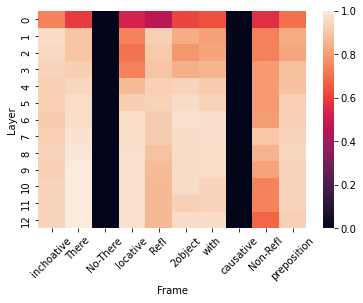
\includegraphics[width=.5\textwidth]{paper/figures/word-heat.png} 
  \caption{Heatmap of the layer performance for contextual word embeddings}
  \label{fig:wordheat}
\end{figure}




The results for the contextual word embeddings, that is, the average embeddings extracted from presenting the sentences in the FAVA datset to BERT, are presented in Table~\ref{tab:contextual-word-results}. We report a comparison with the best-performing BERT layer with the original performance on the CoLA embeddings (repeated from Table~\ref{tab:static-word-results}).  We find that the contextual word embeddings extracted from within the layers of BERT dramatically outperform both the static BERT embeddings and the CoLA embeddings.  Futhermore, we note that, with one curious exception the best performing layers are concentrated around the upper half of the network, from layer $5$ to layer $10$.  The exception is the inchoative frame, whose best-performing layer is layer $1$.  The full performance across all layers is represented in Figure~\ref{fig:wordheat}.




\section{Experiment 2: Sentence-embeddings}
\label{sec:experiment2}

\subsection{Method}
In order to answer the second question: "At the sentence level, do BERT's embedding layers contain the frame and alternation properties of their main verb?", we are going to build a Logistic Regression classifier for each alternation class which will take in a sentence-level embedding extracted from a BERT model and output a binary label: 0 for ungrammatical and 1 for grammatical. To get sentence-level embedding, we average word embeddings across an entire layer for a sentence. Here, we plan to do probing on sentence embeddings on every layer (from the static layer to the final layer) to figure out which layer encodes these related linguistic knowledge. The whole process can be described by the following equation:
$$c_{{s}_{i}} = LR( \textbf{W}\textbf{s}_{i} +\textbf{b})$$

Here, we use (1a) \textit{Janet broke the cup} as an example to explain. $c_{{s}_{i}}$ is a binary value corresponding to whether sentence $s_i$ is grammatical, $\textbf{s}_{i}$ refers to the embedding of the whole sentence \textit{Janet broke the cup}, $LR$ refers to the probe classifier, and $\textbf{W}$ and $\textbf{b}$ are the parameters of $LR$. In this example, $c_{{s}_{i}}$ will be 1, as this sentence is grammatical.
\subsection{Results}
Figure (\ref{fava:mcc}) shows the mcc scores of different BERT layers for each alternation class on the original FAVA datasets. From the figure, we can see that except for the ``understood'' class, there are significant distinctions among these different layers. The trend here is lower layers cannot encode enough related linguistic knowledge. Four of them achieve the best performance on the $9^{\text{th}}$ or  $10^{\text{th}}$ layer, which demonstrates higher layer will encode more information such as the whole sentence structure that will be very useful in judging whether a sentence is grammatical. The ``outlier'' here is ``dative'' class. The best informative layer for ``dative'' is $6^{th}$, after the $6^{th}$ layer, the performance is going down.

Figure (\ref{fava:acc}) shows the accuracy of different BERT layers for each alternation class on the original FAVA dataset. From the figure

 \begin{figure}[htbp]
  \centering
  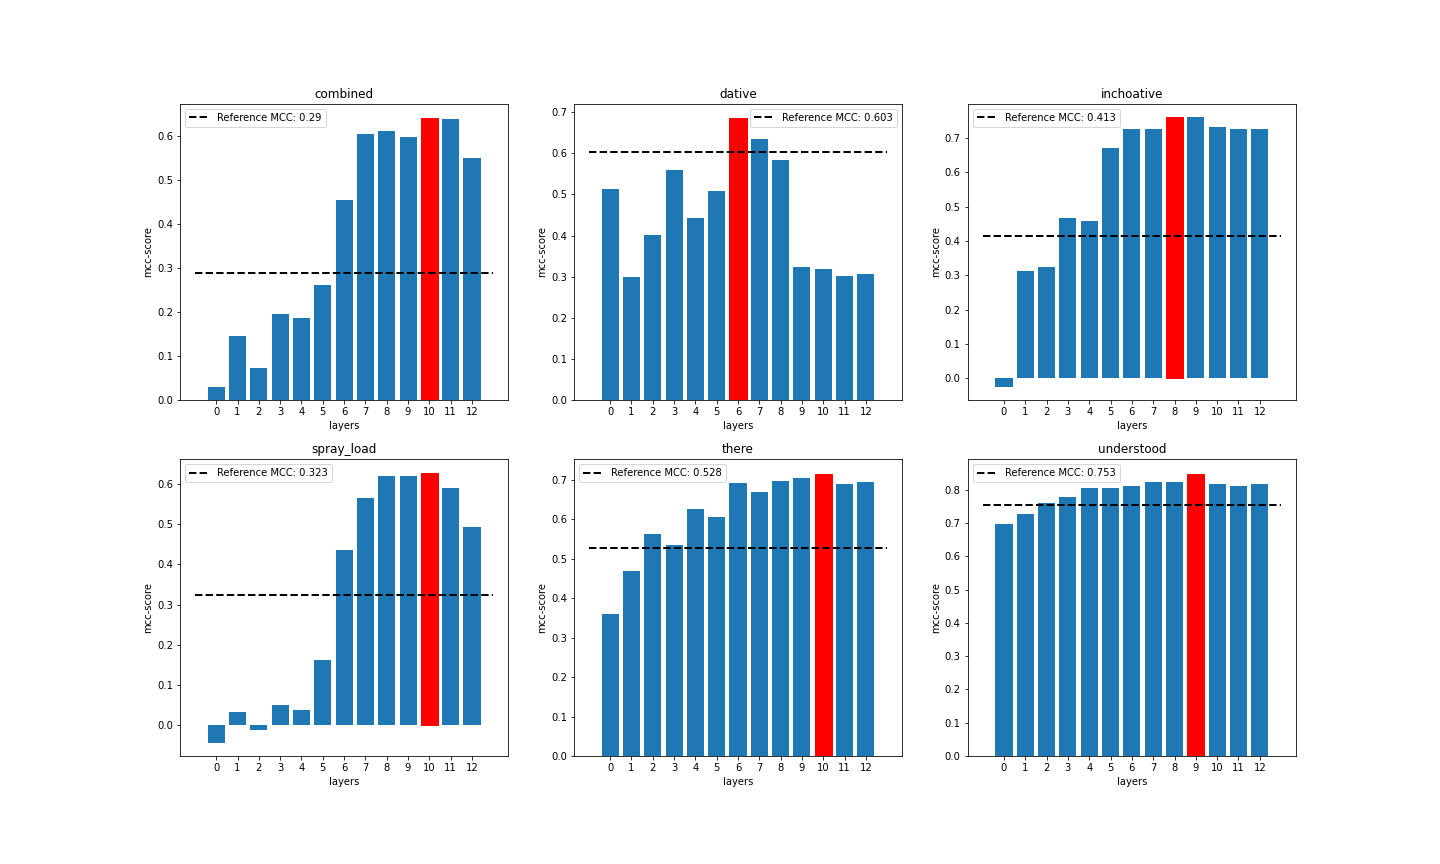
\includegraphics[width=.5\textwidth]{paper/figures/mcc_fava.png} 
  \caption{MCC score for each alternation class on FAVA}
  \label{fava:mcc}
\end{figure}
 \begin{figure}[htbp]
  \centering
  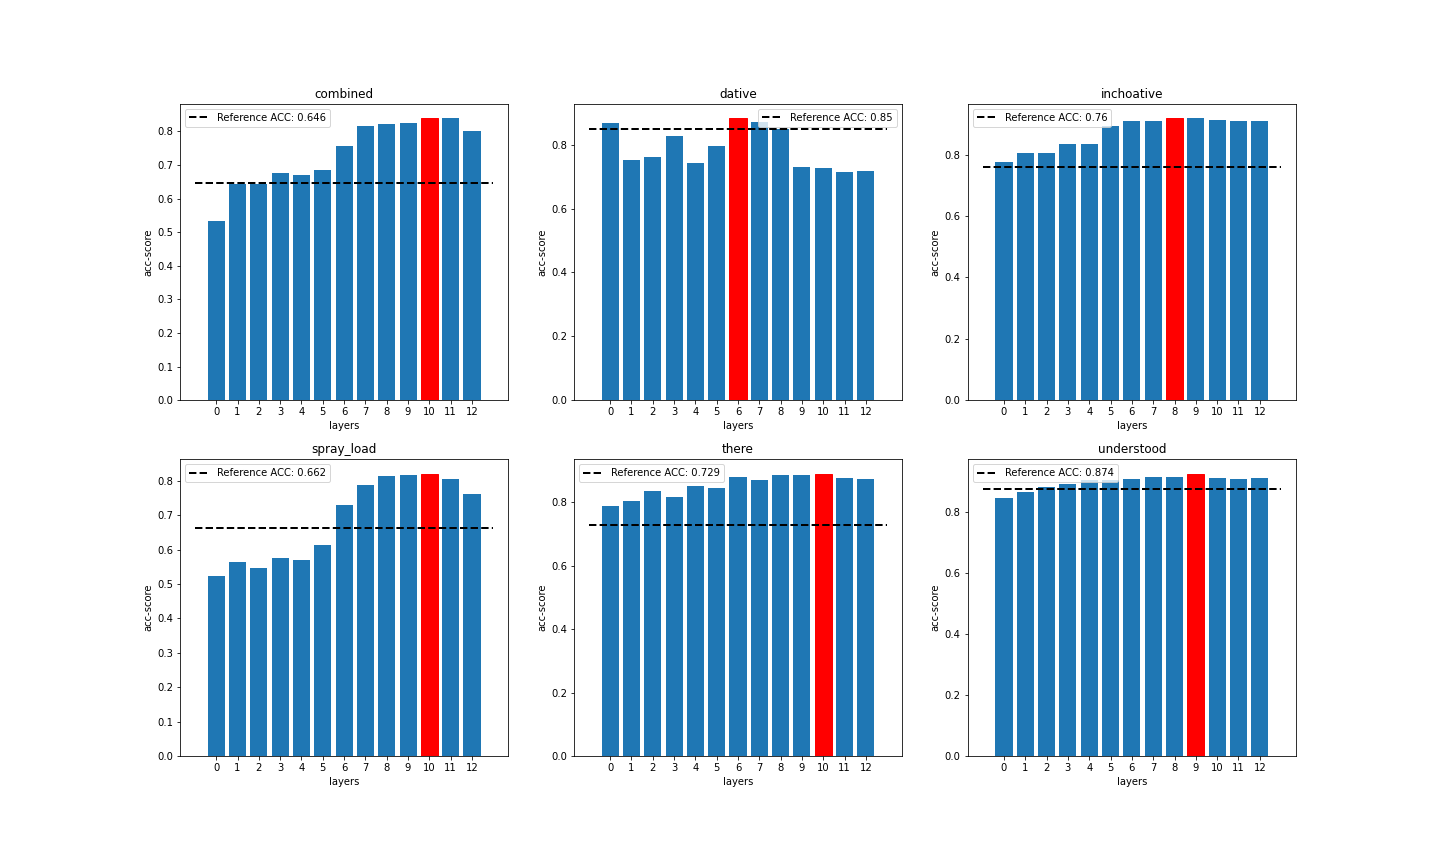
\includegraphics[width=.5\textwidth]{paper/figures/acc_fava.png} 
  \caption{ACC score for each alternation class on FAVA}
  \label{fava:acc}
\end{figure}

% Please add the following required packages to your document preamble:
% \usepackage{multirow}
\begin{table*}[]
\centering
\small
\setlength\tabcolsep{2pt}
\begin{tabular}{cccccccc}\hline\hline\\[1pt]
                             &      & Comb. & CAUSATIVE-INCHOATIVE & DATIVE & SPRAY-LOAD & there-INSERTATION & UNDERSTOOD-OBJECT \\[3pt]\hline\hline\\[0.5pt]
\multirow{2}{*}{BERT}        & MCC  & 0.643 & 0.760                & 0.686  & 0.628      & 0.716             & 0.848             \\[1pt]
                             & Acc. & 84    & 92                   & 88.5   & 82.1       & 89                & 92.5              \\[1pt]\hline\\[0.5pt]
\multirow{2}{*}{GLOVE-based} & MCC  & 0.290 & 0.603                & 0.413  & 0.323      & 0.528             & 0.753             \\
                             & Acc. & 64.6  & 85.4                 & 76     & 66.2       & 72.9              & 87.4              \\[1pt]\hline
\multirow{2}{*}{Majority BL} & MCC  & -     & -                    & -      & -          & -                 & -                 \\
                             & Acc. & 66.6  & 77.6                 & 82.1   & 60.3       & 77.5              & 53.7           \\[1pt] \hline \\[0.5pt]
\end{tabular}
\caption{Results from Experiment 2. For the BERT model, only results from the best layer are reported}
\label{sentence-results}
\end{table*}



\section{Discussion}
\label{sec:discussion}

\begin{itemize}
    \item re: Causative-inchoative performs best at layer 1 vs.~the others which are deeper: causativity may be more of an issue related to the lexical semantics of any given word, whereas the other alternations may be more syntactic in nature.
    
\end{itemize}

\section{Conclusion}
\label{sec:conclusion}


\bibliography{paper}

\appendix

\section{Example Appendix}
\label{sec:appendix}

This is an appendix.

\end{document}
